\section{Introduction}
% abstract + intro fill first page

% information society, modern, communication, integral part of daily life, substantial amounts of data, prior research either topics or networks (not both)

% heuzutage viele daten als graph
% gibt spezielle dbs (neo4j)
% ein problem graphähnlicher daten: überblick
% netzdaten twitter, social media, semantic web
% kontext emails
% weg von bloß knoten/kanten -> 
In our modern information society we produce substantial amounts of data each day.
A large portion of it comes from the communication on social media platforms or through emails.
Special graph databases enable the efficient storage of these large communication networks and provide interfaces to query or analyse the data.
Visualising networks in their entirety on the other hand is a very challenging task.
Users investigating a document collection want to find information about \textit{when} does \textit{who} talk \textit{to whom} about \textit{what}.

Given the communication data over a year or more, it is practically impossible to gain an overview or quick insights into the latent network structure with a basic approach as shown in \Fref{fig:netvis}.
Also, in such a traditional \textit{network visualisation}, information about the content of messages sent between individuals is lost.
Besides these traditional systems, more exotic approaches use the metaphor of geographical maps~\cite{pang2017creating} to visualise networks, for example using topology to reflect connectivity of densely connected social communities.
The map analogy can also be used to visualise the contents of documents by embedding them into a high dimensional semantic space~\cite{le2014distributed} and projecting it on the map as a \textit{document landscape}.
In order to highlight how relationships form and change based on the interactions, the metaphor of a growing tree ca be used (ContactTrees~\cite{sallaberry2016contact}).
Although this reflects temporal aspects of dynamic networks well, it focuses on one person as the root, thus an overview of the entire network is lost.
CactusTrees~\cite{dang2017cactustree} on the other hand represent hierarchical structures with the goal of untangling overlaid bundles of intersecting edges, making distant connections more apparent.
As higher order dependencies may get lost in traditional visualisations, HoNVis~\cite{tao2017honvis} adds nodes to encode dependencies in chains of interactions.
Usually, a communication network has many nodes and overlapping connections already, so Yang et al.~\cite{yang2014overlapping} rather focus on discovering overlapping cores to improve the identification of community boundaries to highlight global latent structures.
Similarly, Gronemann et al.~\cite{gronemann2012drawing} use the metaphor of islands and hills to visualise clustered graphs, making densely connected communities clearly noticeable.
The edges are bundled and follow valleys of the resulting topology, thus making relationships between other communities hard to follow.
MapSets~\cite{efrat2015mapsets} assume a graph that was laid out using embeddings reflecting communities.
An algorithm then draws regions around clusters of nodes, such that the bounding shapes are contiguous and non-overlapping, but yet abstract.
Another approach to visualise networks at full scale is to aggregate nodes based on their spatial distribution and thereby allowing for a simple exploration with contour lines and heatmap overlays to emphasise latent structures as proposed by Hildenbrand et al.~\cite{hildenbrand2016flexible}.

% ==== GRAPH VIS ====
%\cite{dang2017cactustree}
%visualization technique for representing hierarchical datasets, specific goal of untangling overlaid bundles of intersecting edges.
%\cite{sallaberry2016contact}
%highlight how relationships form and change based upon interactions among actors, as well as how relationships and networks vary by contact attributes
%
%\cite{tao2017honvis}
%higher order visualisation of network by adding (splitting) nodes to encode higher-order dependencies (ie conditional probability), Objective: (ie) discover ports relevant for species invasion, extract higher order dependencies (ie not pairwise, but tuple of len 3 -> cond prob of last node given first node)
%\cite{yang2014overlapping}
%discover overlapping "cores" in network graph for more accurate communities and improved identification of community boundaries
%
%\cite{gronemann2012drawing}
%clustered graph as map with islands
%\cite{efrat2015mapsets}
%visualising embedded+clustered graphs, find regions, how to map them out nicely
%\cite{hildenbrand2016flexible}
%aggregates nodes based on their spatial distribution, thereby allowing for visual exploration of large graphs, contour lines/heatmap

\begin{figure*}[tp!]
	%	\centering
	\begin{tikzpicture}[]
	\node[draw,anchor=north west,inner sep=1] at (0,0) {%
		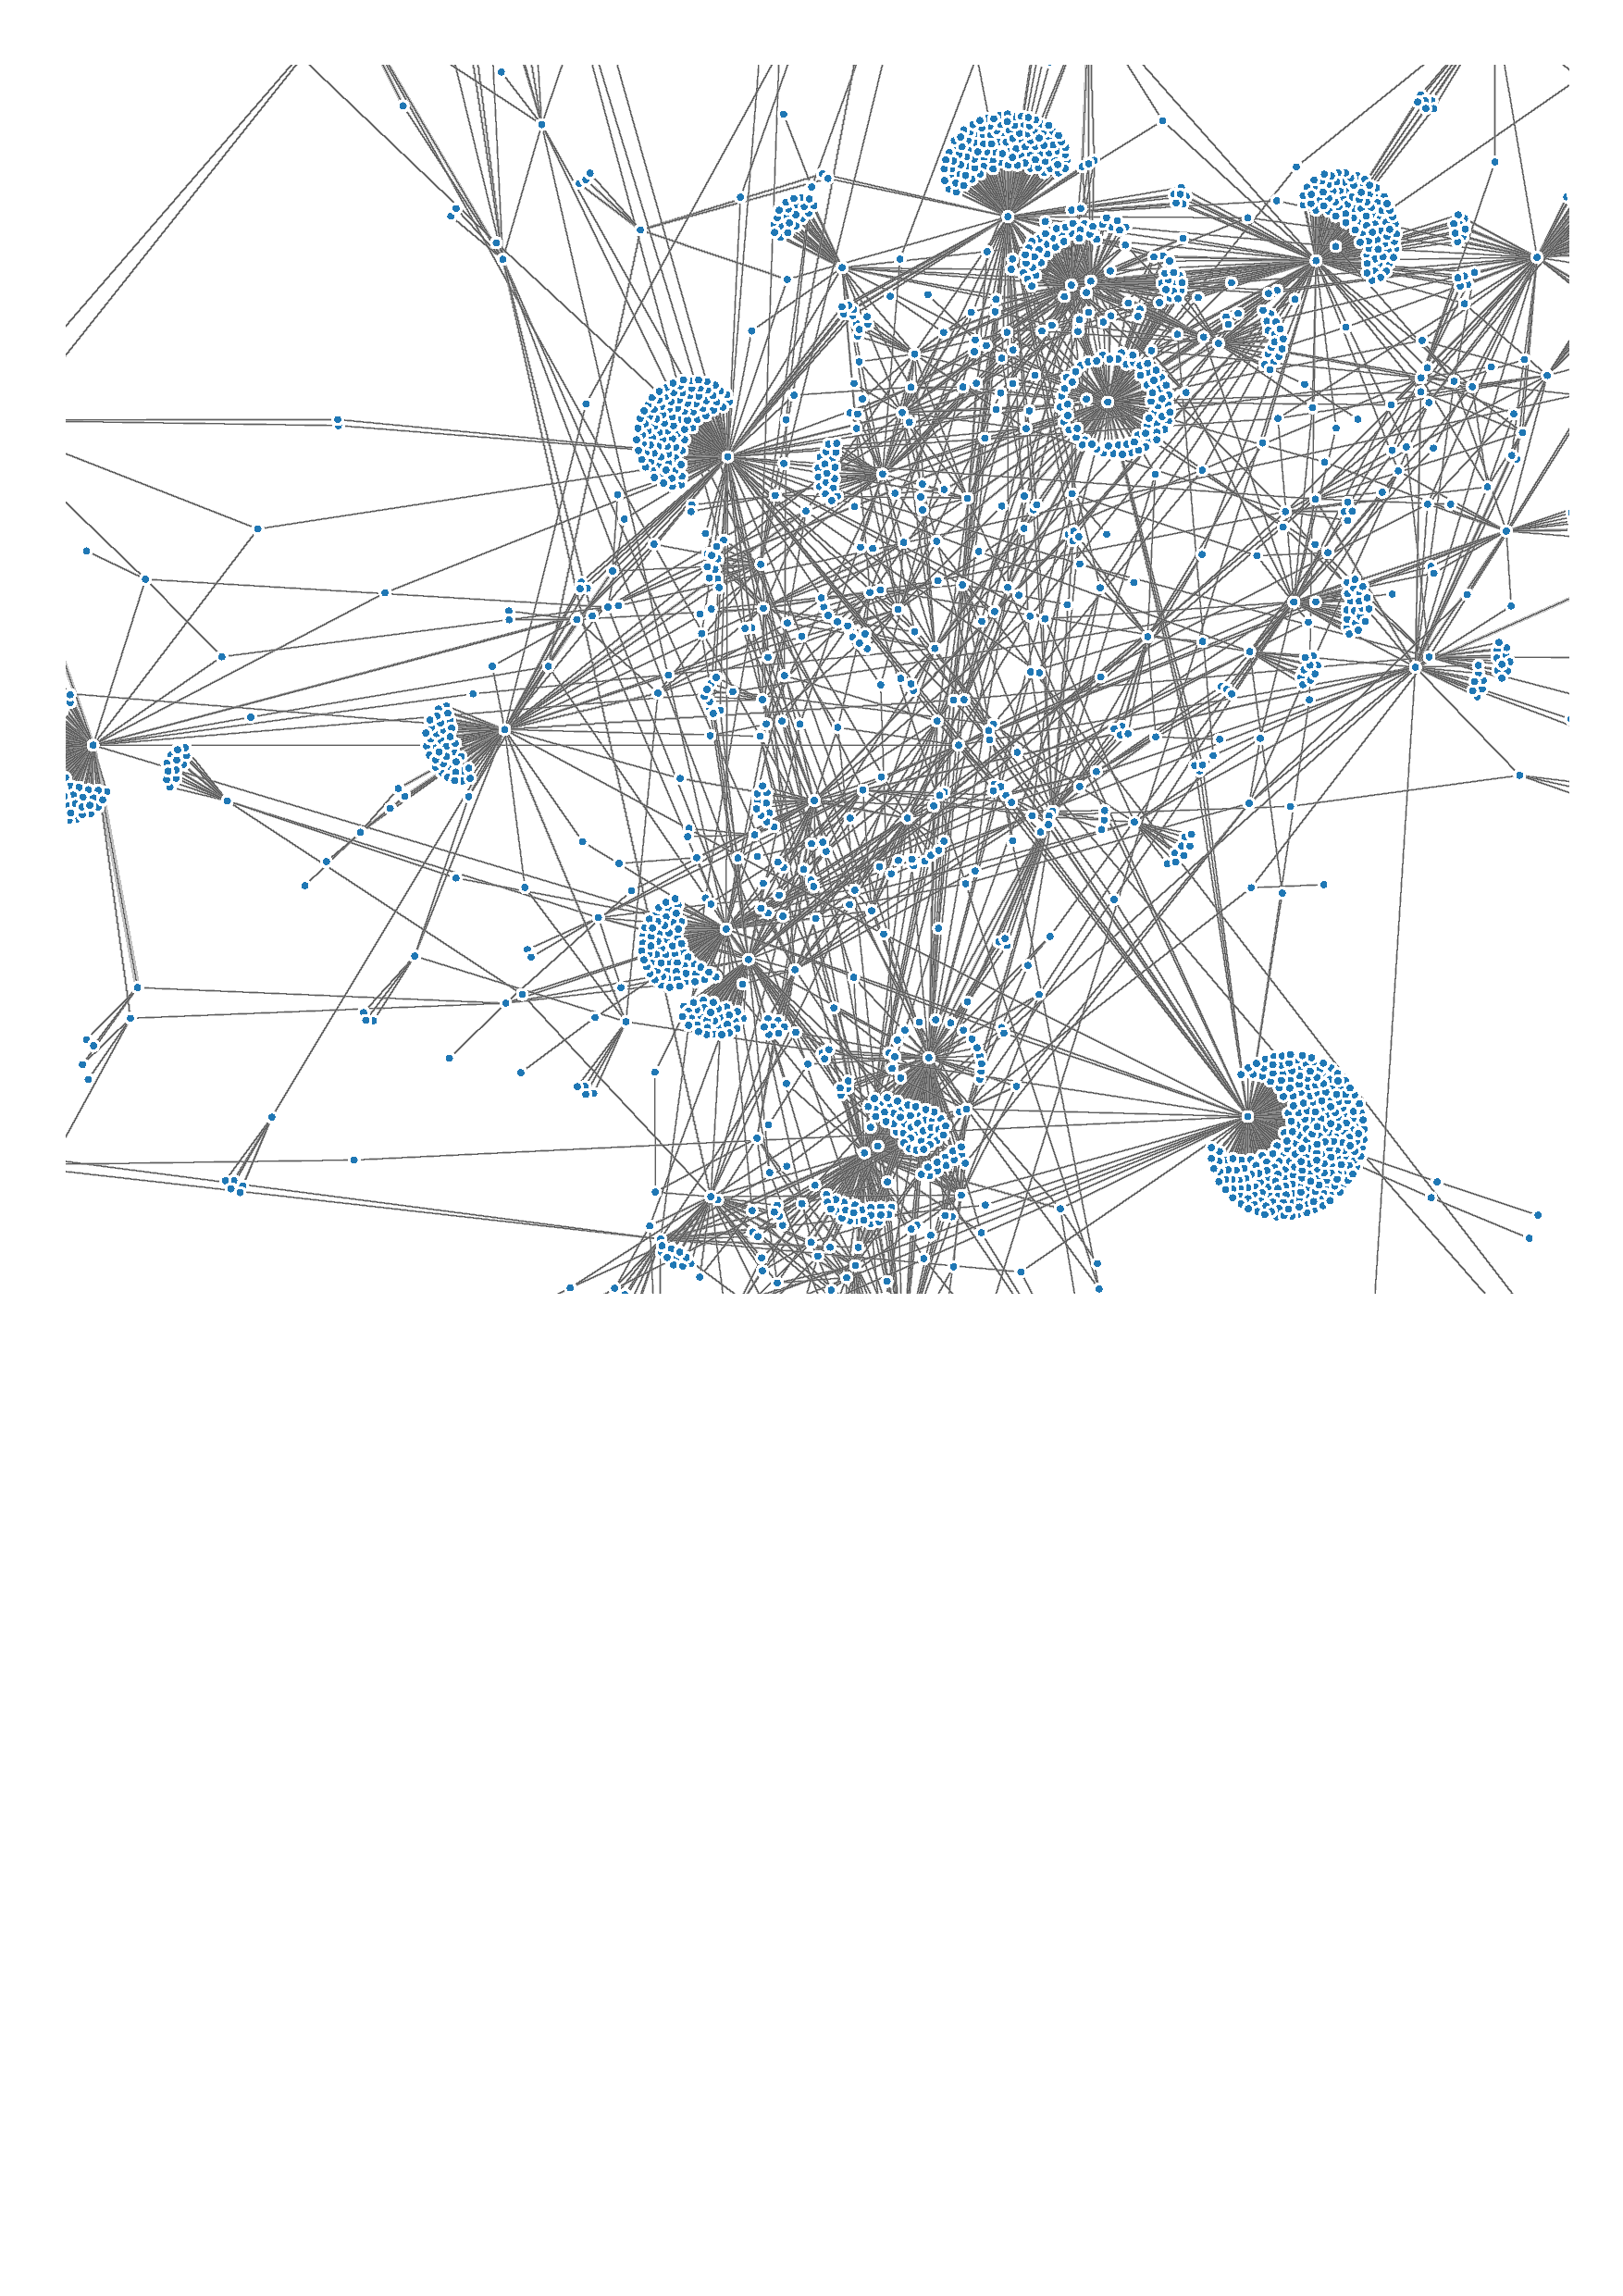
\includegraphics[%
		trim={8cm 32.5cm 1cm 4cm},% left bottom right top
		clip,%
		width=0.8\textwidth]{network}%
	};%
	\end{tikzpicture}
	\caption{Traditional basic visualisation of a communication graph from 2000 emails using force layout}
	\label{fig:netvis}
\end{figure*}


\textit{Document visualisation} aims to visualise the content, such that users gain quick insights into topics, latent phrases, or trends.
Tiara~\cite{wei2010tiara} extracts topics and derives time-sensitive keywords to depict evolving subjects over time as stacked plots.
Other approaches project documents into a latent space, using topic models or embeddings.
Creating scatter-plots of embedded documents of a large corpus may result in a very dense and unclear layout, so Chen et al.~\cite{chen2009exemplar} developed an algorithm to reduce over-full visualisations by picking representative documents.
A different approach is taken by Fortuna et al.~\cite{fortuna2005visualization}, who do not show documents directly, but generate a heatmap of the populated canvas and overlay it with salient phrases at more densely populated areas from the underlying documents in that region.
Friedl et al.~\cite{fried2014maps} extend that concept by drawing clear lines between regions and colouring them.
They also add edges between salient phrases based on co-occurrences in the texts.
Most recently Cartograph~\cite{sen2017cartograph} was proposed, which is visually very similar to previous approaches, but uses pre-rendered information of different resolution and map technology to enable a responsive interactive visualisation.
Regions are coloured based on underlying ontologies from a knowledge-base.

Our goal is to \textit{merge approaches for network and document visualisations} in one interactive user interface.
Giving an overview over latent structures and topics in one map may significantly improve the exploration of a corpus by users unfamiliar with the domain and terminology.
Application scenarios that could benefit from such a multi-dimensional view include investigative journalists and auditing firms.

% === TEXT VIS ===
%\cite{wei2010tiara}
%Extract topics and derive time-sensitive keywords to depict the content evolution of each topic over time visualised as stacked plots
%\cite{chen2009exemplar}
%pick exemplars to reduce over-full visualisation (scatter plot)
%\cite{fortuna2005visualization}
%visualise text corpus (heatmaps + dots for docs + salient phrases)
%\cite{fried2014maps}
%maps of computer science, similar but draws clear regions and edges reflecting co-occurrence
%\cite{sen2017cartograph}
%Visualisation System for thematic maps that position Concepts (ie Named Entities) into semantic space on map, pre-render and use maps technology

% 
%\cite{wang2016linked}
%which combines link and label information with content information to learn document representations for classification
%\cite{goyal2017graph}
%graph embedding survey
%\cite{bikakis2016exploration} 
% visual exploration of big liked semantic data - challenges


%related work
%\begin{itemize}
%	\item two parts: network vis, textvis
%	\item embeddings: doc2vec, node2vec
%	\item hierarchical/level of detail
%	\item map semantic
%	\item cartograph close to us, but no network
%	\item highlight missing link between text and network in all research
%\end{itemize}

%introduce topic, challenges, rough goal, related work

\section{Interactive Visualisation}
% this section fills second page (inkl mockup)
% describe objectives and what data is available and how that can be used
Systems for document exploration largely vary in what they display and how users interact with them.
This depends partly on the available raw data, but also on information extracted from pre-processing or enrichment with external sources.
\Fref{fig:netvis} shows a basic visualisation of the network graph extracted from an email corpus.
Although it is an improvement over only listing connections, large densely connected graphs quickly become hard to read and information about the email contents is lost.

Exploring document collections can be seen as a top-down approach, where the system provides abstract overviews of the entire document collection and users incrementally refine the search, narrowing the results to just a few documents of interest.
Such a top-down approach may help users without prior knowledge to get a sense for the data by visualising high level latent structures of communication networks or the topical distributions.

In the scope of this work we primarily consider documents to be emails or data attached to them.
The sender, recipients, time, and content can directly be extracted from the raw data.
We call these -- and results from further processing -- \textit{dimensions} that can be visualised.
From the contents one may infer named entities, topics, embeddings, or salient phrases, while the communication network spanned by sender-recipient pairs can be used to detect salient structures and hierarchies.
The temporal information enables the previously mentioned data to be analysed over time to detect evolving or changing patterns.

There are numerous ways to visualise each dimension on its own or in combination with others.
The requirement of a dimension and its priority in a visualisation is dictated by the system objective.
From the wide range of possibilities, we strive for a system which supports the exploration of a large collection of documents without any prior knowledge about its content and individuals involved.

In our system, we use the names and email addresses of senders and recipients (\textit{individuals}), communication network, semantic vector representations of email contents, and as part of an overlay the timestamps of emails and propose a graph layout over a document landscape that visually describes \textit{who} talks \textit{with whom} about \textit{what} at a given \textit{time period}. 

\begin{figure*}[th!]
	%	\centering
	\begin{tikzpicture}[]
	\node[draw,anchor=north west,inner sep=1] at (0,0) {%
		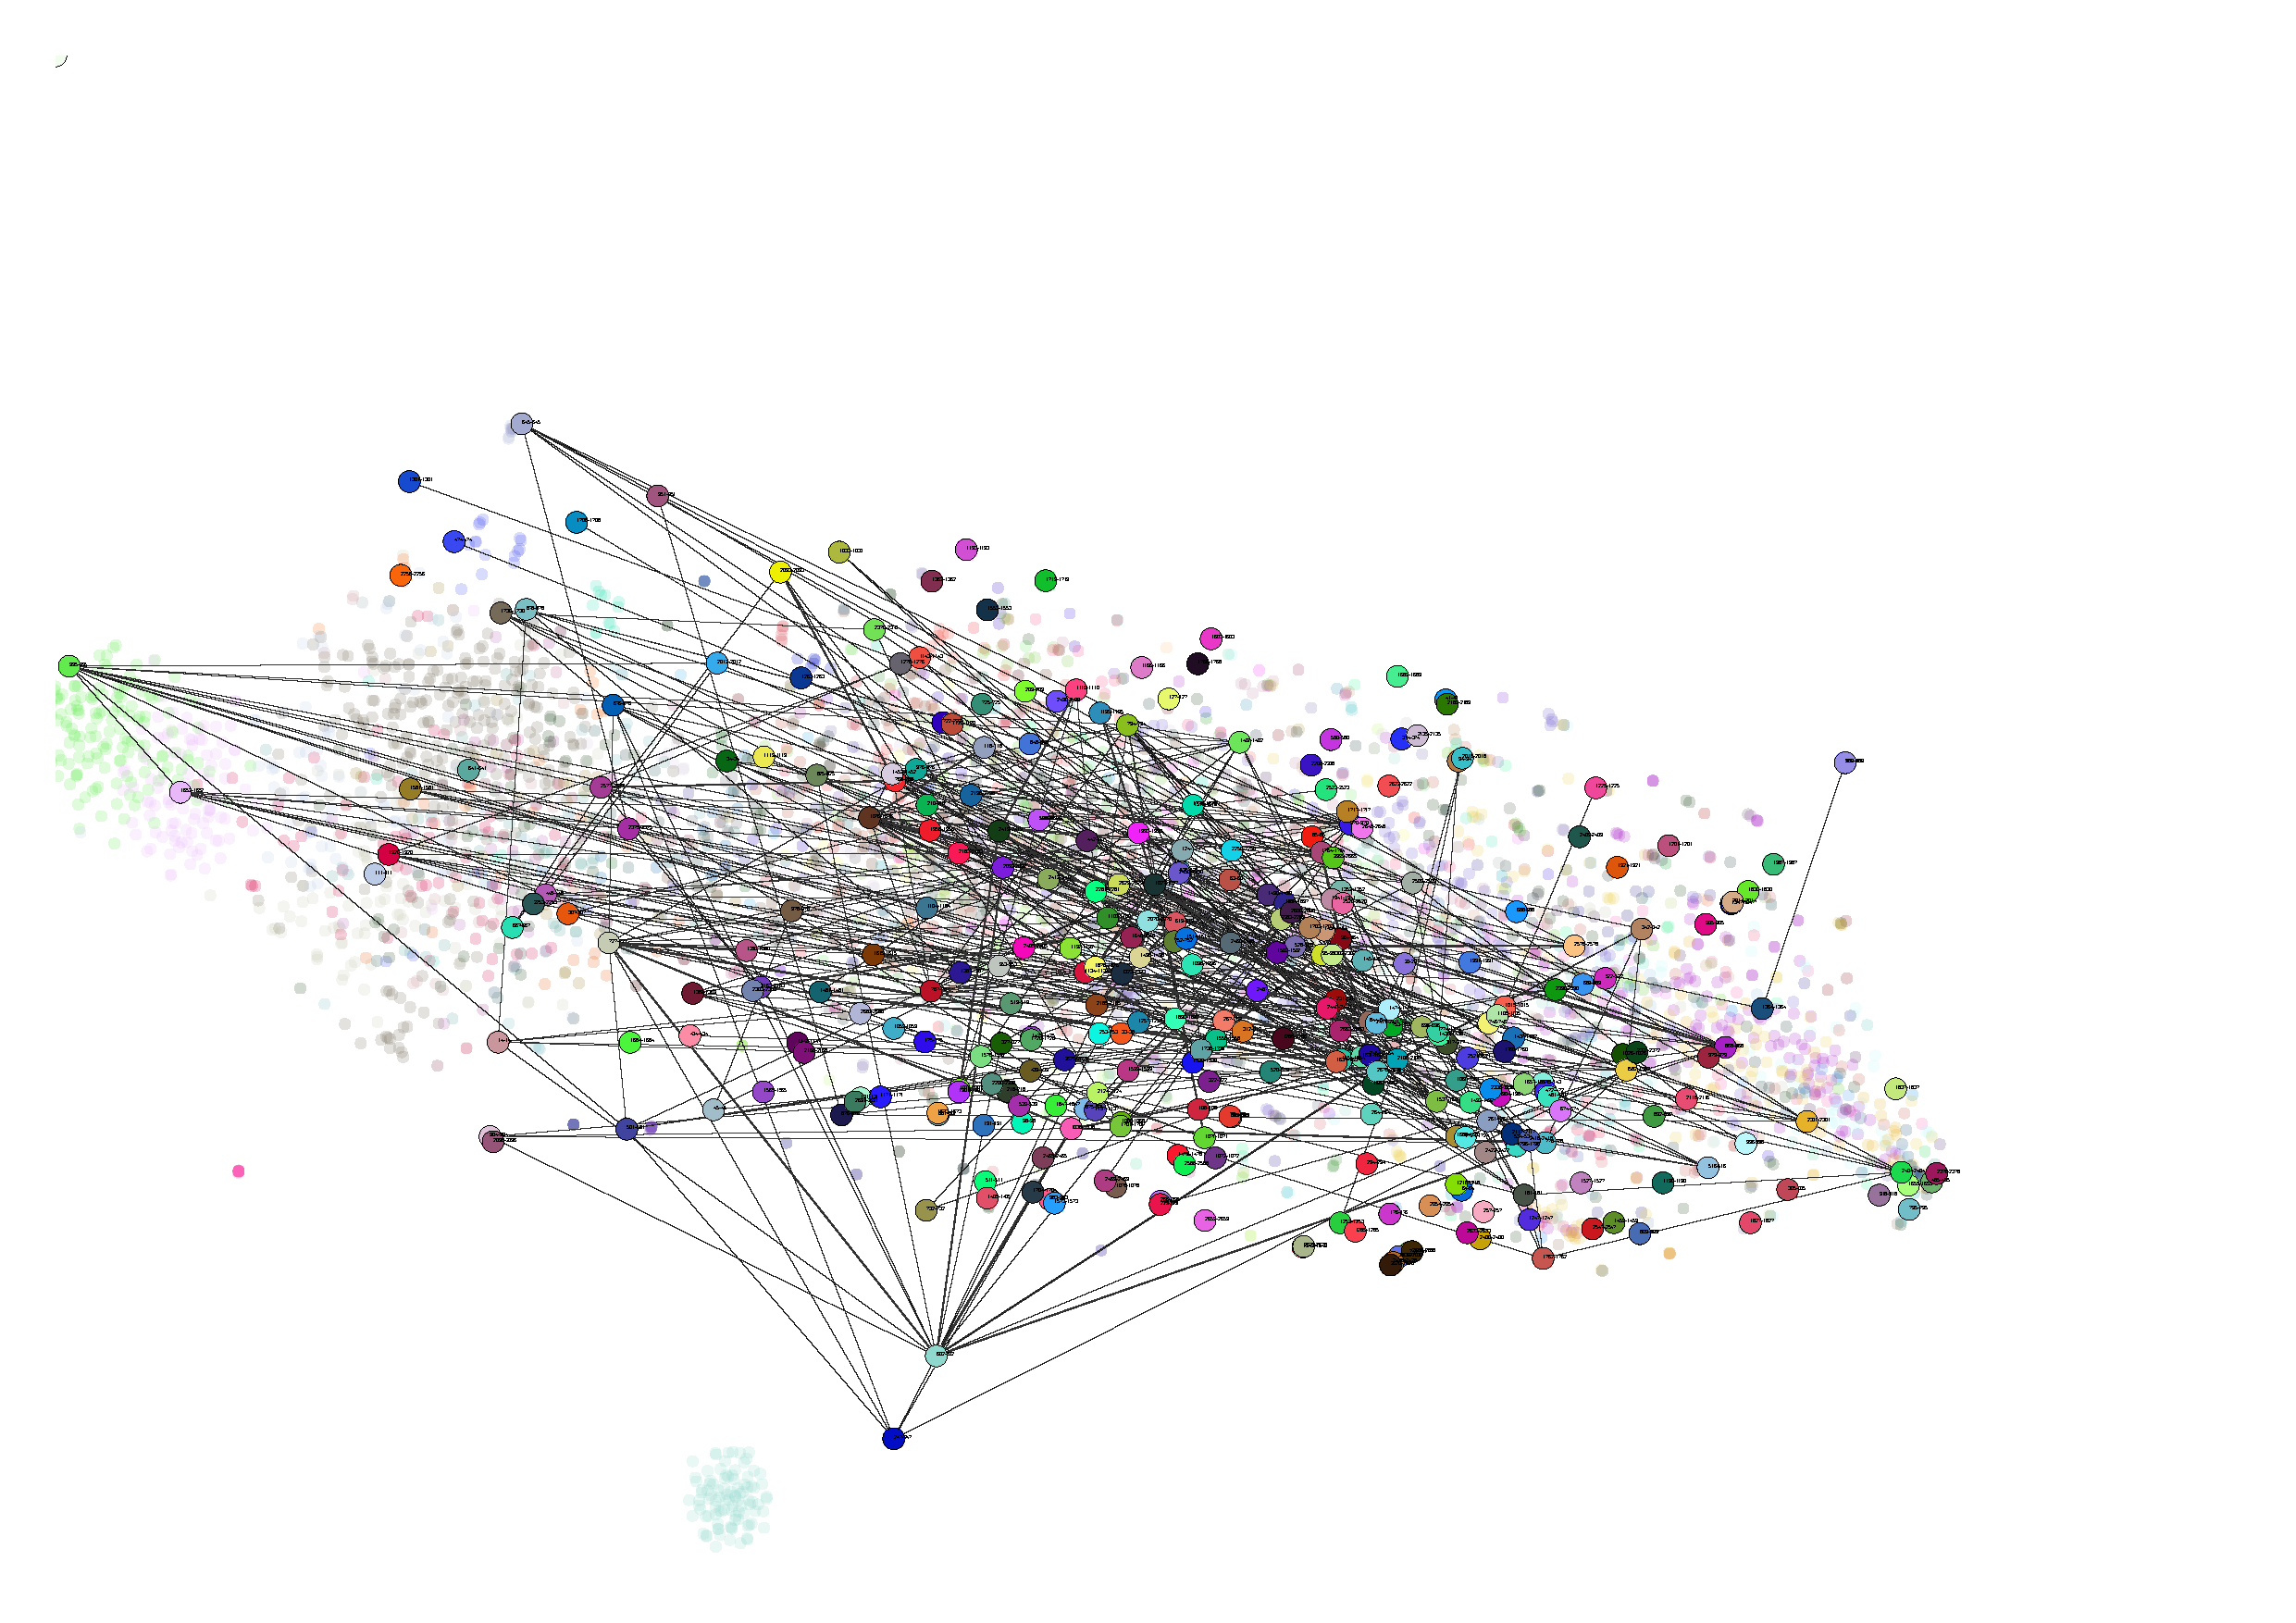
\includegraphics[%
		trim={1cm 14cm 20cm 10cm},% left bottom right top
		clip,%
		width=0.8\textwidth]{poc}%
	};%
	\end{tikzpicture}
	\caption{Rendered prototype output after landscape initialisation without prior community segmentation}
	\label{fig:poc}
\end{figure*}

%We further distinguish between domain oriented and open systems. 
%A domain oriented system may have specific vis, extract, ext data,...


\section{System Architecture}
% fills full page 3 and max the first half of left column page 4
%describe concrete system and outline algorithmic approach
Visualising communication networks in a topic-aware fashion to explore documents and salient structures is not straightforward
Different layout objectives may produce contradicting results and the challenges of processing big data need to be addressed~\cite{bikakis2016exploration}.
In this section, we describe algorithmic approaches behind the system we are working on.
For a discussion of engineering aspects on how to store, serve, and render the map-like data, we refer to the Cartograph~stack~\cite{sen2017cartograph}, as we will focus on the process how to get the information that the map is generated from.
% self citation -> quagga for preprocessing?

We visualise the embedded emails as dots in a two-dimensional landscape in which individuals are placed as nodes connected by edges.
All emails between two individuals are reduced into one edge reducing visual complexity and making it easier to detect salient structures.
However, that comes with the trade-off that nodes and edges cannot be perfectly placed in the landscape to cover all semantic aspects of the communication between them, but rather an estimate.
Our very early prototype placed some individuals with no dominant topic in a crowded area in the centre of the landscape as shown in \Fref{fig:poc}, where colours of opaque dots for emails correspond to that of the sender.
Although the network visualisation at this point does not make connections more clear than in \Fref{fig:netvis}, users can already distinguish individuals with similar or unrelated topics.

Our proposed algorithm to find a stable network layout has three stages, namely an \textit{(i) initialisation phase} which creates the landscape and roughly places nodes and connections, an \textit{(ii) update phase} which iteratively updates the node placement towards a better fit, and finally a \textit{(iii) post processing phase} where edges become splines to make latent structures more clear and a map topology is added.

% == ALGORITHM ==
% global doc2vec
% node2vec
% community detection (threshold)
% use each community center to populate landscape with selection of community's emails 
%   -> tsne on doc2vec
% place nodes at avg doc2vec of sent mails
% calculate each persons ideal line (lin reg) in landscape
% calculate neighbourhood similarity between nodes within communities
% minimise loss function
% edge bundling
% map topology


%One na\"ive approach to combine a flat visualisation of the document embedding space and communication graph is to assume the embedded emails to be fixed and place the nodes of the graph close to where most emails are projected to.
%This way, many edges may cross each other and communities can't be visually distinguished.
%Furthermore, in case emails of an individual contain two dominant subjects which are far apart in the semantic space, ideal placement of the node becomes ambiguous.

%We assume, that the communication between two individuals 

%optimise towards
%stable balance

\paragraph{Initialising the Landscape.}
To generate the document landscape, we first process the network graph to roughly determine regions, where documents will be placed.
Therefore we apply node2vec~\cite{grover2016node2vec} to the communication network and embed each individual's node.
We separate the graph into communities $P_i\subset P$ using the kernel density of the resulting populated space at threshold $\kappa$, where a higher $\kappa$ results in more, but smaller communities.
For each community $P_i$, pairwise neighbourhood similarities are calculated using euclidean distance between nodes, forming the triangular matrix $S_i$, where $s_{kl}$ is the similarity between $p_k,p_l\in P_i$.

Furthermore, we train document embeddings~\cite{le2014distributed,hu2017} on all emails and use them to infer high dimensional semantic vector representations.
Let $M_i$ be the set of emails that originated in community $P_i$.
For each email $m\in M_i$, the dimensionality is reduced using t-SNE~\cite{maaten2008visualizing}, which retains possible semantic clusterings of documents in the higher dimensional space.
The resulting two-dimensional vectors are then placed as dots on the map using the centre of embedded network communities as the respective origin, whereas the size is determined by the number of related individuals.

We also initialise communication network's layout.
Thereby, the staring position of a node representing an individual is determined by the normalised sum of two-dimensional vectors of all emails he or she has sent or received.
This way, we implicitly group semantically related individuals into communities as frequent communication biases this normalised sum.
Straight edges are added between the nodes if the respective individuals exchanged emails.
Note, that many edges may only represent a small number of emails.
Applying a variable threshold $\sigma$ can reduce the computational load in later stages, as these edges will not impact the overall layout very much.
They can be added again as the user requests a detailed visualisation by zooming in or through other interactions.

In the algorithm's second stage, we iteratively try to improve the layout of the communication network by finding a balance between the closeness of nodes to semantic context and densely connected neighbourhoods a node belongs to.
Therefore, for each individual $p_j\in P$ we use linear regression to fit a line $\widehat{m_{p_j}}$ though all two-dimensional vectors of emails he or she has sent or received.
As a node is placed near this line, it remains in a semantically good position.

\paragraph{Adjusting the Network Layout.}
The first stage of our proposed algorithm produces a fixed document landscape and roughly fits the communication network on top. 
We now aim to incrementally adapt the layout of the graph to better reflect salient structures in the network while keeping each individual's node close to the reflective semantic area in the landscape.

Therefore we define a score quantifying how well the current layout fits these objectives:
\begin{equation}
\sum_{p_i\in P}
\bigg[
\eta~d(p_i, \widehat{m_{p_i}})+
%\sum_{\substack{p_j\in P\\p_i\sim p_j}}
\sum_{p_j\in P}
\theta\left(s_{ij}-d(p_i,p_j)\right)
\bigg]
\label{eq:score}
\end{equation}
where $d(\cdot,\cdot)$ is the distance between two nodes (zero if no connection exists) or shortest distance from a node to its ideal line.
To adjust the layout towards either a better semantic or structural fit, we introduce parameters $\theta$ and $\eta$.

%\begin{figure}
%	% alternatively use teaserfigure (manual page 18)
%	% A special kind of figure is used for many two-column conference proceedings. This figure is placed just after the authors, but before the main text. The environment teaserfigure is used for these figures. This environment must be used before \maketitle
%	\dummyfig{0.15}{0.2}{post init example}
%	\dummyfig{0.15}{0.2}{post layout example}
%	%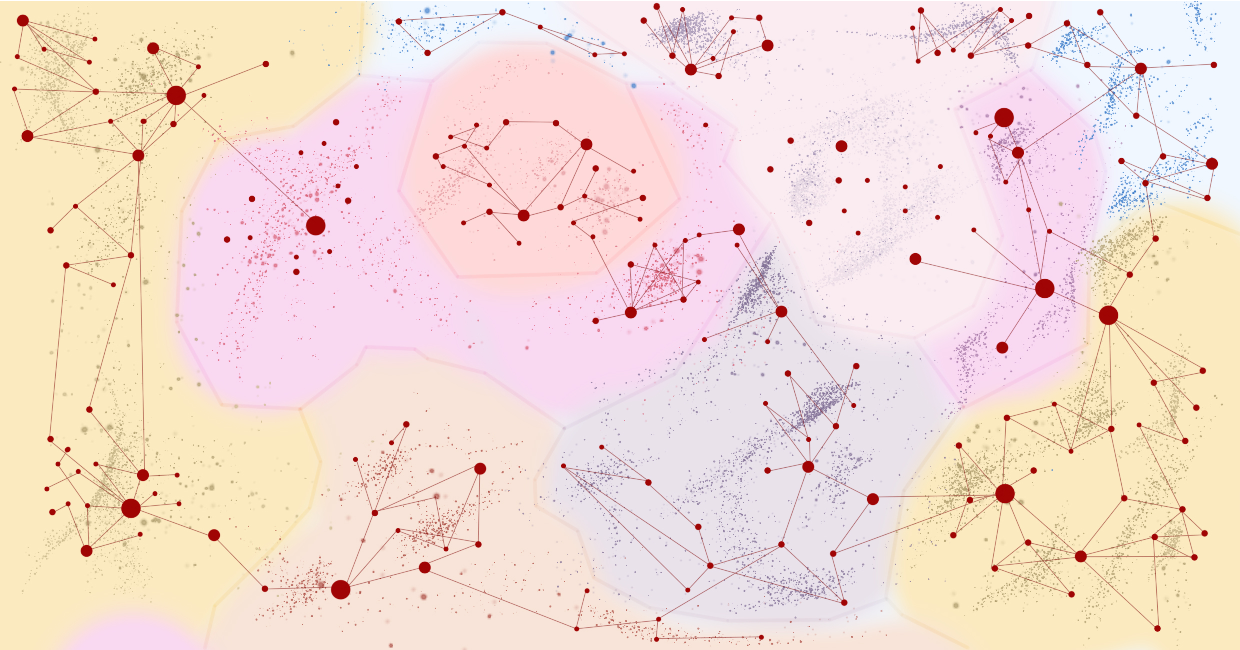
\includegraphics[width=0.9\textwidth]{mockup2}
%	\caption{Schematic example after initialisation (left) and after layout optimisation (right). Nodes and edges of the graph are blue, green dots are embedded emails, dotted lines are email--edge relationships, arrows are update vectors}
%	\label{fig:minisample}
%\end{figure}

%\Fref{fig:minisample} schematically shows a small possible scenario after initialisation.
%There, the network layout does not yet reflect our objectives very well as communities are spread apart and mixed.
%We incrementally move the nodes towards a stable minimum of \Fref{eq:score}.

In order to minimise \Fref{eq:score}, we use stochastic gradient descent.
In each iteration step, we can derive the direction and magnitude each node should be moved towards a better semantic fit and closer proximity to it's neighbourhood in the network.

The semantic gradient for $p_j\in P$ is defined by
\begin{equation}
\vec{\delta^s_j}:=  (p_j^m - p_j)~\lVert p_j^m - p_j\rVert
\label{eq:ds}
\end{equation}
where $p_j^m$ is the closest point on $\widehat{m_{p_j}}$ to $p_j$ and $\lVert\cdot\rVert$ denotes the euclidean norm, while neighbourhood gradient is defined by
\begin{equation}
\vec{\delta^n_j}:= \sum_{\substack{p_k\in P\\p_j\sim p_k}}(p_j - p_k)~\left(\lVert p_j - p_k\rVert - s_{jk}\right)
\label{eq:dn}
\end{equation}
where $p_j\sim p_k$ denotes that an edge exists between $p_j$ and $p_k$.

With the definitions in \Fref{eq:ds} and \Fref{eq:dn}, we can formulate the update vector $\vec{\delta_j}$ for node $p_j\in P$ as
\begin{equation}
\vec{\delta_j}:=\xi\left(\theta\vec{\delta^n_j}+\eta\vec{\delta^s_j}\right)
\label{eq:dj}
\end{equation}
where $\xi$ is the learning rate and $\theta,\eta$ as before parameters to weight between a better semantic or neighbourhood fit.

Most likely, complex network structures might prevent the stochastic gradient descent to find a stable minimum, so the score of the objective function should be monitored or intermediate layouts be visually evaluated to determine a satisfactory result.

\begin{figure*}[th!]
	%	\centering
	\begin{tikzpicture}[]
	\node[draw,anchor=north west,inner sep=1] at (0,0) {%
		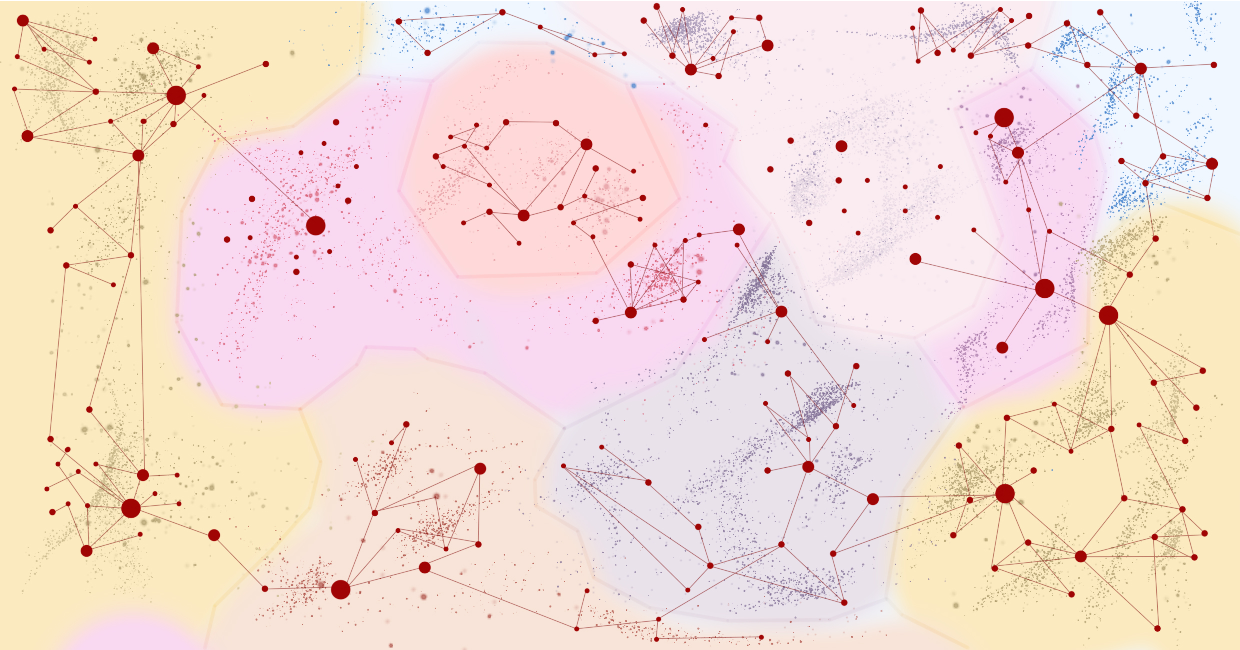
\includegraphics[%
		trim={0 4.5cm 0 0.5cm},% left bottom right top
		clip,%
		width=0.8\textwidth]{mockup2}%
	};%
	\end{tikzpicture}
	\caption{Semantic landscape of email contents and dominant communication patterns (drawn mockup)}
	\label{fig:mockup}
\end{figure*}

\paragraph{Post Processing.}
Lastly, we use the post processing stage to enhance the readability of our visualisation.
Densely connected communities in the graph are potentially hard to read, thus we apply edge bundling~\cite{bach2017towards} to visually clear latent structures.
We also apply MapSets~\cite{efrat2015mapsets} to separate the regions for each community.
Since semantically similar emails may appear in different communities, we apply colouring based on clusters in the original global document embedding space to retain this aspect.
Choosing the colours depends on the number of latent topics that should be depicted~\cite{zeileis2009escaping}.
If the topic number exceeds 25-30 topics, grouping topics and allowing for zooming within a two-level topic-hierarchy ensures distinguishable colors for up to 10 subtopics ($25 \times 10=25$).
In order to represent temporal aspects of the data, we calculate the kernel density of the document landscape for fixed time-intervals, which can be used to add heat-map overlays that users can select later on. 

% bend and bundle edges , calculate network "topology" (community density as heatmap or topological lines), colour the graph (using topic clustering in case layout isn't close to landscape or community colouring if communities aren't visually close enough -> future research)

%parts of the system: prep, server, frontend
%\begin{itemize}
%\item node2vec
%\item node clustering/communities
%\item doc2vec
%\item tsne for docs in cluster
%\item find stable layout
%\item calculate metric for node importance
%\item calculate metric for salient phrases
%\item use last three for map generation with zoom levels
%\item mapserver, database, leaflet (see cartograph)
%\end{itemize}
%
%describe idea of fully neural approach: feed doc2vec and node2vec to second stage network, use that representation only; discuss outcome (nice because fully semantic and no intervention, bad because outcome unpredictable and potentially visually not practical)

\section{Conclusion and Vision}
In the previous sections, we described an algorithm to lay out a communication network on top of a landscape of semantically embedded emails.
This is still work in progress, so \Fref{fig:mockup} shows a manually drawn mock-up of the visualisation we aim for to visually convey our vision.
In it, individuals are represented as nodes positioned such that densely connected communities are visually clustered.
Edges describe the email traffic, where the opacity and thickness is used to indicate the frequency of messages between the nodes they connect.

The semantic representations of emails are used to place dots on a background layer which we call the \textit{document landscape}.
This landscape is used as additional input to the graph layout algorithm, aiming to place a node within corresponding semantic regions.
The colouring of regions in the landscape is derived from densely connected communities in the communication graph.

Optionally, representative words are selected for densely populated areas in the landscape, so that users get a rough idea about subjects in that area.
The aforementioned timestamps of emails can be used to generate a heatmap overlay to show the activity in a certain time interval which is controlled by a slider.

Similar to modern geographical maps, zooming into a region reveals more details.
In our case, less prominent individuals and their connections are shown along with additional salient phrases from the document landscape.
Selecting a node will not only highlight connected edges but may also temporarily show more edges which were previously hidden at that zoom level.
The user will also be able to retrieve documents with the help of a selection rectangle or clicking dots in the document landscape.

In future work, we hope to evaluate this system using full-scale real-world data.
It may also be interesting to experiment with embedding methods, which take both the emails and the network graph as input and directly project the inferred representations into the two-dimensional landscape to simplify the proposed algorithm.

We belief that such a system enables users to quickly gain an overview of relationships between communicating individuals and their semantic context.
This approach may for example help journalists to not only get an initial understanding of large amounts of leaked data, but also help them later on for in-depth investigations.

% fills left column on page 4, right column mostly references
%\begin{itemize}
%	\item nice app of big data to find salient communication structures in semantic space
%	\item highlight contribution (combine network vis and text vis)
%	\item future: implement it, refine algorithm, evaluate usefulness
%\end{itemize}
